\section{Introduction to Reinforcement Learning from Human Feedback (RLHF)}
\label{sec:intro-rlhf}

Reinforcement Learning from Human Feedback (RLHF) is a method that 
uses human feedback to better align model-generated outputs with human preferences. 
In its most basic form, RLHF involves training a model to generate text that aligns with human 
preferences \footnote{human preference here is defined as a text that is 
is more helpful, less biased, and less toxic} \cite{ouyangTrainingLanguageModels2022, zhengSecretsRLHFLarge2023, 
yangFoundationModelsDecision2023}.

\subsection{Overview of Large Language Models (LLMs)} \label{subsec:llms}

LLMs are a class of AI models that are trained to generate text. These models
are trained in three key phases: Pre-training, Supervised Fine-Tuning (SFT), and 
Reinforcement Learning from Human Feedback (RLHF) \cite{ouyangTrainingLanguageModels2022}.

\subsubsection{Phase 1: Pre-training} \label{subsubsec:pre-training}

In the Pre-training stage, the goal is to encode statistical information about the language by processing 
vast amounts of text data. For simplicity, statistical information here means how 
likely a word appears after another word (given the context).
For native speakers, this is an easy task, because they unconsciously have the statistical knowledge
of the language. For example , given the sentence  \textit{"My favorite car brand to drive is..."
}, the language model would give higher probability for the word "Audi" than the word "Banana".
A visual explanation of this process is available on the \href{https://poloclub.github.io/transformer-explainer/}
{Transformer Explainer}.

\begin{figure}[h]
    \centering
    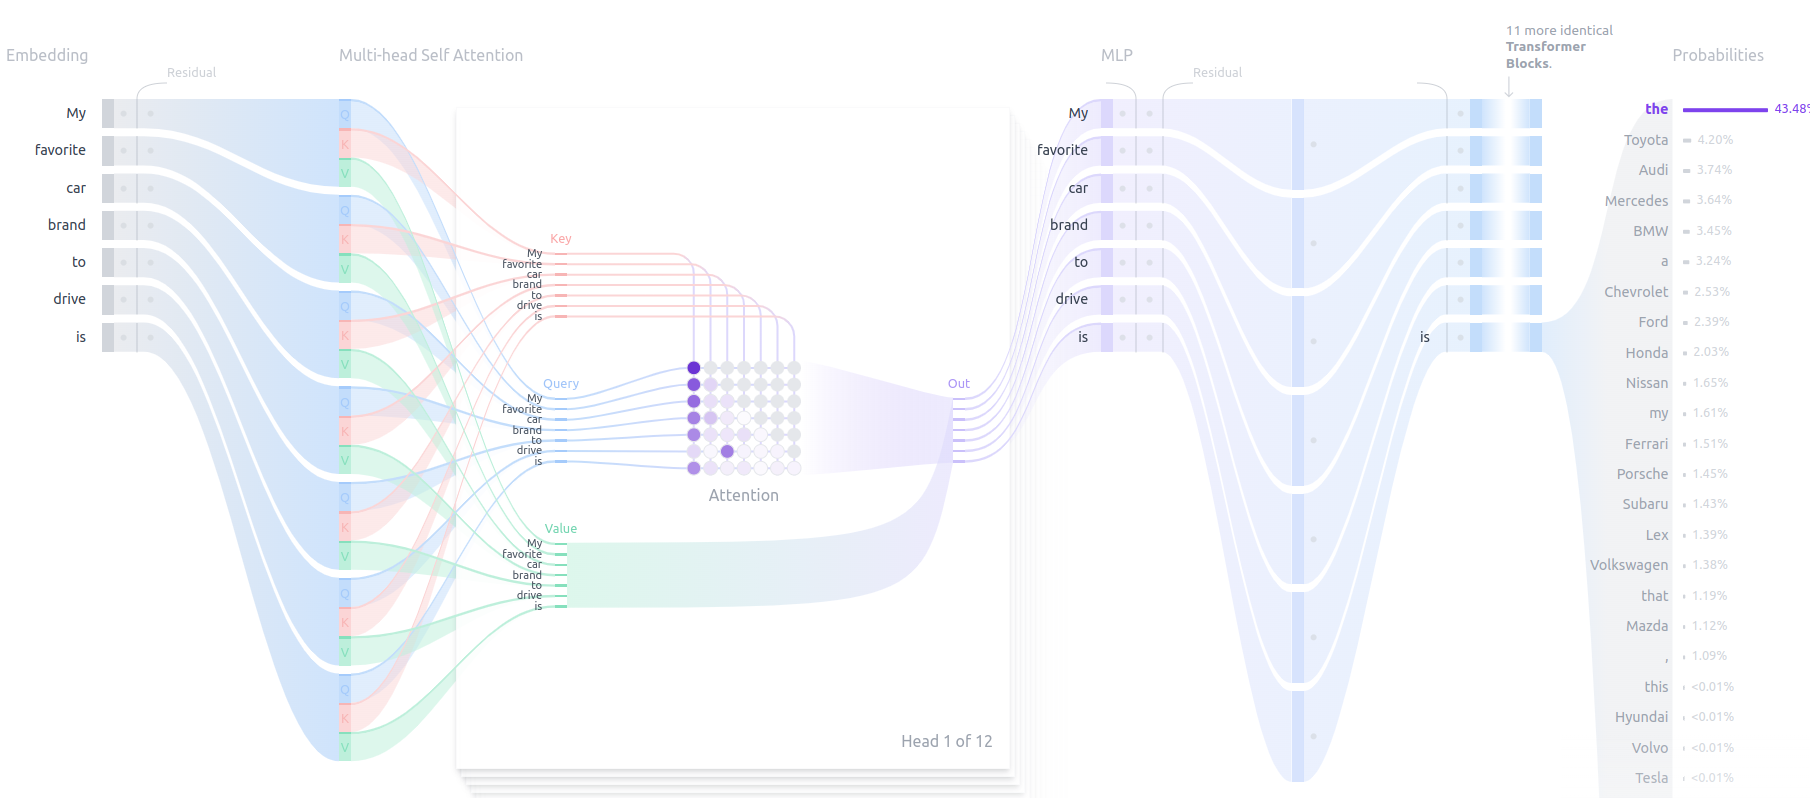
\includegraphics[width=1\textwidth]{./figures/transformer.png}
    \caption{An example visualization from the Transformer Explainer website.}
    \label{fig:transformer-explainer}
\end{figure}

In the example shown in the Figure \ref{fig:transformer-explainer}, the model receives the input text 
(on the left side with Embedding column) and generates probabilities 
for the next word, which are visualized on the far right of the plot. 
s demonstrated, the token "the" has the highest probability of occurrence, 
followed by "Toyota" and "Audi".



While pre-training stage helps LLMs with getting broad statistical knowledge of the language, 
it has two significant limitations:


\begin{itemize}
    \item Flexibility of Text: text completion has a very flexible nature, 
    the goal is not to complete the the text, rather to be useful for user. 
    Therefore, post pre-training stages are needed to make language models "useful".
    \item Toxicity and Bias: Pre-trained models often reflect biases present in the training data, 
    make them to generate harmful and biased texts \cite{ouyangTrainingLanguageModels2022}.
\end{itemize}


\subsubsection{Phase 2: Supervised Fine-tuning (SFT)} \label{subsubsec:sft}

In Phase 1, we trained a language model to complete the sentences. 
But conversations have a very flexible structure and can be completed in many different ways. 
For example, given the prompt "How to travel from Paris to New York?", 
there can be several possible answers. Some of the possible answers are:

\begin{itemize}
    \item while sleeping and watching TV
    \item with most excited view
\end{itemize}

So, here, we want to further fine-tune the pre-trained model using supervised training 
so that, given a 'prompt,' it produces a 'response' that aligns with our objectives. The goal of this phase of the training is to help the model learn to prioritize the responses that are more helpful, like:

\begin{itemize}
    \item The best way is to travel is by airplane, with flights available daily.
\end{itemize}

So, here we enter the world of "Supervised learning" where we have a “Prompt” and a “Response” (label), 
to train the model. For example, during the development of InstructGPT \cite{ouyangTrainingLanguageModels2022}, 
OpenAI employed 40 labelers via Upwork to curate approximately 13,000 "Prompt-Response" pairs, 
commonly referred to as demonstration data. As example, Figure \ref{fig:demonstration-data} shows
an example of demonstration data used in Supervised Fine-tuning. (three prompts and three responses 
provided by human labelers).


\begin{figure}[h]
    \centering
    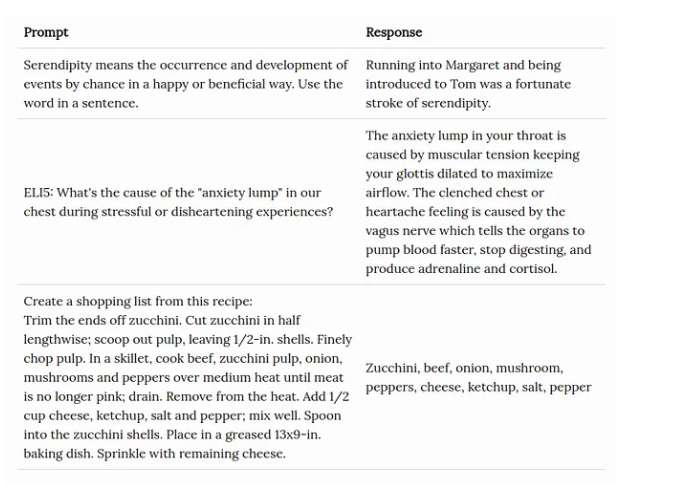
\includegraphics[width=0.6\textwidth]{./figures/dmonstartondata.png}
    \caption{An example of Demonstration data used in Supervised Fine-tuning.}
    \label{fig:demonstration-data}
\end{figure}

The main objective of supervised fine-tuning (Phase 2) is to further fine-tune the pre-trained model 
to generate responses that closely align with user needs, using the human-generated demonstration data.

\subsubsection{Phase 3: Reinforcement Learning from Human Feedback (RLHF)} \label{subsubsec:rlhf}

The final stage of training LLMs involve Reinforcement Learning (RL). 
The idea here is how to involve "human" feedback in training the LLMs to enhance the model's 
output alignment with human preferences. Texts have a quite flexible nature, 
and the goal is how to make text generate by LLMs more
\textbf{helpful}, \textbf{less-biased} and \textbf{less-toxic}. 
\cite{ouyangTrainingLanguageModels2022}, 
In other words, human feedback is believed to improve LLMs by providing intuition 
for complex tasks that are difficult to formalize and automate. Empirically, 
RL has been shown to enhance the performance of the SFT model Phase 2. 

For example, as shown in Figure \ref{fig:instruct}, 
LLMs with only 1.3B (billion) parameters trained using RLHF were 
preferred over a 175B parameter model trained using Supervised Fine-tuning (SFT). 
This preference suggests the effectiveness of RLHF in enhancing model
performance beyond what can be achieved with SFT alone.


\begin{figure}[h]
    \centering
    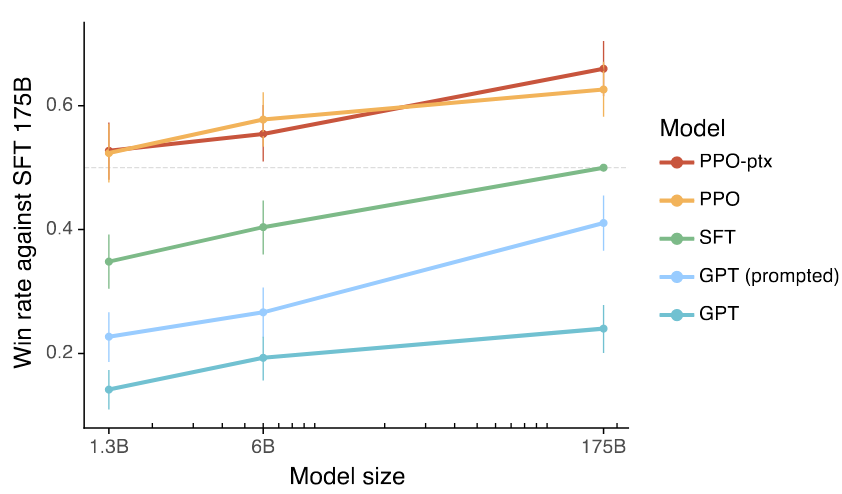
\includegraphics[width=0.8\textwidth]{./figures/instruct.png}
    \caption{Comparison of model performance with and without RLHF (orange and red lines are RLHF), 
    source \cite{ouyangTrainingLanguageModels2022}}
    \label{fig:instruct}
\end{figure}


In the next section, it is discussed how RL framework can contribute to improving LLM performance. To address this, 
we begin by examining the foundational components of the RL framework.

\subsubsection{Reinforcement Learning (RL) Framework} \label{subsec:rl-framework}


The RL framework consists of three main components: \textbf{State}, \textbf{Action}, and \textbf{Reward}. 
These components form the basis for RL frameworks, which are used to train agents to interact with
environments and learn to maximize expected cumulative rewards. In the context of LLMs, the three components
need to be defined as follows:

\begin{itemize}
    \item \textbf{Action}: 
        \begin{itemize}
            \item Based on the policy, the agent will make an action derived from the policy. In LLMs, 
            the action is to generate the next token (completion to the prompt), 
            derived from the policy.
        \end{itemize}
    \item \textbf{State}: 
        \begin{itemize}
            \item The agent receives a state from the environment (i.e., the dialogue history). In 
            LLMs, the state consists of all the dialogue text up to this point 
            (both by the agent and the human).
        \end{itemize}
    \item \textbf{Reward}: 
        \begin{itemize}
            \item The environment returns a reward, \( r(s_t, a_t) \), which is calculated from a 
            reward function trained from human preference data. In the context of the LLMs,
            we do not have direct access to rewards, but we can build a reward model trained from 
            human preferences \cite{christianoDeepReinforcementLearning2017}.
        \end{itemize}
\end{itemize}

The RL framework is illustrated in Figure \ref{fig:rlhf-process}.
The objective of reinforcement learning (RL) is to derive a policy that 
maximizes the cumulative reward. In the context of large language models 
(LLMs), the concept of "reward" is nuanced. Specifically, we seek to determine the 
reward through human feedback, which evaluates the quality of the model's responses to given 
prompts. This feedback helps in identifying whether the generated responses are good, bad, or helpful.


\begin{figure}[h]
    \centering
    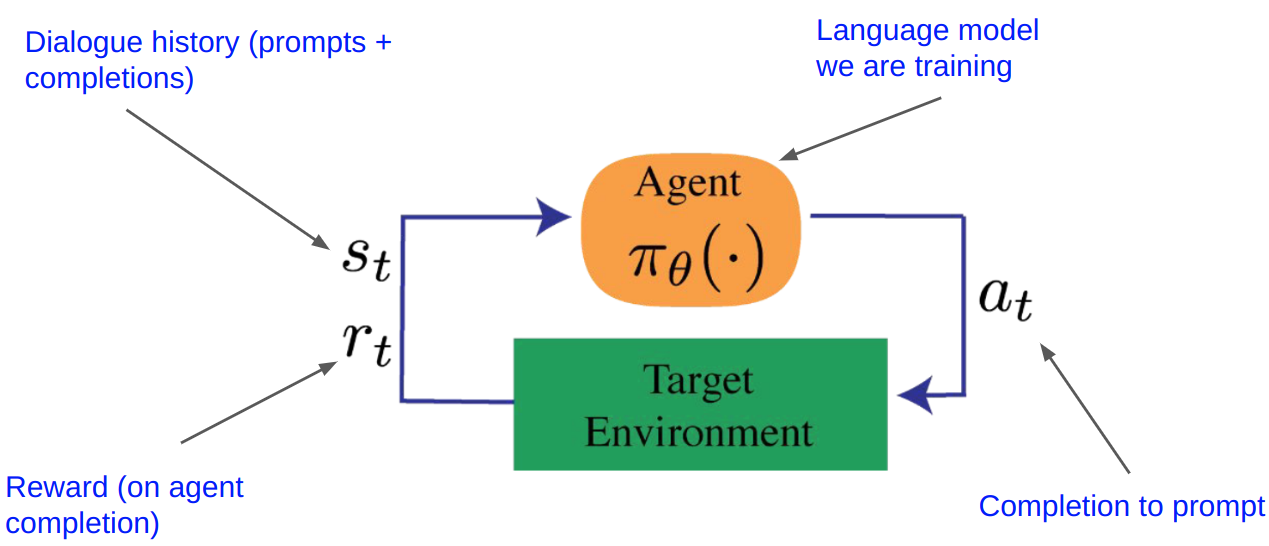
\includegraphics[width=0.8\textwidth]{./figures/rlhf_1.png}
    \caption{An illustration of the Reinforcement Learning from Human Feedback (RLHF) process. \cite{lambertBasicsReinforcementLearning}}
    \label{fig:rlhf-process}
\end{figure}